\documentclass[answers]{exam}
\usepackage{marvosym}

%...TikZ & PGF
\usepackage{pgfplots}
\pgfplotsset{compat=1.11}
\tikzset{>=latex}
\usetikzlibrary{calc,math}
\usepackage{tikzsymbols}
\usepgfplotslibrary{fillbetween}
\usetikzlibrary{decorations.markings} 
\usetikzlibrary{arrows.meta} %...APP2 for arrows as objects and images
\usetikzlibrary{backgrounds} %...For shading portions of graphs
\usetikzlibrary{patterns} %...Unit 5 Problems
\usetikzlibrary{shapes.geometric} %...For drawing cylinders in Unit 2
\tikzset{
    mark position/.style args={#1(#2)}{
        postaction={
            decorate,
            decoration={
                markings,
                mark=at position #1 with \coordinate (#2);
            }
        }
    }
} %...See https://tex.stackexchange.com/questions/43960/define-node-at-relative-coordinates-of-draw-plot

\tikzset{
    declare function = {trajectoryequation10(\x,\vi,\thetai)= tan(\thetai)*\x - 10*\x^2/(2*(\vi*cos(\thetai))^2);},
    declare function = {trajectoryequation(\x,\vi,\thetai)= tan(\thetai)*\x - 9.8*\x^2/(2*(\vi*cos(\thetai))^2);},
    declare function = {patheq(\x,\yi,\vi,\thetai)= \yi + tan(\thetai)*\x - 9.8*\x^2/(2*(\vi*cos(\thetai))^2);},
    declare function = {patheqten(\x,\yi,\vi,\thetai)= \yi + tan(\thetai)*\x - 10*\x^2/(2*(\vi*cos(\thetai))^2);} %like patheq but with gravity = 10
}

%...siunitx
\usepackage{siunitx}
\DeclareSIUnit{\nothing}{\relax}
\def\mymu{\SI{}{\micro\nothing} }
\DeclareSIUnit\mmHg{mmHg}
\DeclareSIUnit{\mile}{mi}
%...NOTE: "The product symbol between the number and unit is set using the quantity-product option."

%...Other
\usepackage{amsthm}
\usepackage{amsmath}
\usepackage{amssymb}
\usepackage{cancel}
\usepackage{subcaption}
\usepackage{dashrule}
\usepackage{enumitem}
\usepackage{fontawesome}
\usepackage{multicol}
\usepackage{glossaries}
%\numberwithin{equation}{section}
\numberwithin{figure}{section}
\usepackage{float}
\usepackage{twemojis} %...twitter emojis
\usepackage{utfsym}
\newcommand{\R}{\mathbb{R}} %...real number symbol
\usepackage{graphicx}
\graphicspath{ {../Figures/} }
\usepackage{hyperref}
\hypersetup{colorlinks=true,
    linkcolor=blue,
    filecolor=magenta,
    urlcolor=cyan,}
\urlstyle{same}
\newcommand{\hdashline}{{\hdashrule{\textwidth}{0.5pt}{0.8mm}}}
\newcommand{\hgraydashline}{{\color{lightgray} \hdashrule{0.99\textwidth}{1pt}{0.8mm}}}

%...Miscellaneous user-defined symbols
\newcommand{\fnet}{F_{\text{net}}} %...For net force
\newcommand{\bvec}[1]{\vec{\mathbf{#1}}} %...bold vector
\newcommand{\bhat}[1]{\,\hat{\mathbf{#1}}} %...bold hat vector
\newcommand{\que}{\mathord{?}}  %...Question mark symbol in equation env
%...Define thick horizontal rule for examples:
\newcommand{\hhrule}{\hrule\hrule}
\let\oldtexttt\texttt% Store \texttt
\renewcommand{\texttt}[2][black]{\textcolor{#1}{\ttfamily #2}}% 

%...For use in the exam document class
\newif\ifprintmetasolutions


%...Decreases space above and below align and gather enironment
\makeatletter
\g@addto@macro\normalsize{%
  \setlength\abovedisplayskip{-3pt}
  \setlength\belowdisplayskip{6pt} 
}
\makeatother





\usepackage[margin=1in]{geometry}
\usepackage[figurewithin=none]{caption}
\usepackage{exam-randomizechoices}

\CorrectChoiceEmphasis{\color{red}\bfseries}
\renewcommand{\solutiontitle}{\noindent\textbf{\textcolor{red}{Solution:}}\enspace}

\usepackage{OutilsGeomTikz}
\usepackage{utfsym} %...Symbols in Unit 7 Problems
\usepackage{tabu} %...Symbols in Unit 7 Problems

%...For use in Unit 2            %    
\setlength{\columnsep}{2cm}      %
\setlength{\columnseprule}{1pt}  %
\usepackage[none]{hyphenat}      %
%%%%%%%%%%%%%%%%%%%%%%%%%%%%%%%%%

%...For use in Unit 11 on Waves:
\pgfdeclarehorizontalshading{visiblelight}{50bp}{  %
color(0.00000000000000bp)=(red);                   %
color(8.33333333333333bp)=(orange);                %
color(16.66666666666670bp)=(yellow);               %
color(25.00000000000000bp)=(green);                %
color(33.33333333333330bp)=(cyan);                 %
color(41.66666666666670bp)=(blue);                 %
color(50.00000000000000bp)=(violet)                %
}                                                  %

\newcommand{\checkbox}[1]{%
  \ifnum#1=1
    \makebox[0pt][l]{\raisebox{0.15ex}{\hspace{0.1em}\Large$\checkmark$}}%
  \fi
  $\square$%
}
%%%%%%%%%%%%%%%%%%%%%%%%%%%%%%%%%%%%%%%%%%%%%%%%%%%%

%...If using circuitikz package:
% \ctikzset{bipoles/battery1/height=0.5}
% \ctikzset{bipoles/battery1/width=0.25}
% \ctikzset{bipoles/resistor/height=0.15}
% \ctikzset{bipoles/resistor/width=0.4}


\setrandomizerseed{1}
\bracketedpoints

\setlength{\columnsep}{2cm}
\setlength{\columnseprule}{1pt}
\usepackage[none]{hyphenat}

\firstpageheader{Physics}{Unit 2: Force Interactions}{Practice Quiz}
\runningheader{}{}{}

\begin{document}
\begin{questions}

\question %...originally in unit 5: force analysis
The free body diagram below represents the forces acting on the box in the image beside it. Given the scenario in the image, which force is missing from the free body diagram?

\begin{randomizechoices}[norandomize]
    \correctchoice frictional force
    \choice weight force
    \choice tension force
    \choice normal force    
\end{randomizechoices}


\question
The graph below shows the velocity of a car that is moving in a straight line.

\begin{center}
    \begin{tikzpicture}
        \begin{axis}[width=7cm,
            height=5cm,
            xmin=0,xmax=50,
            ymin=0,ymax=35,
            xlabel={Time (s)},
            ylabel={Velocity (m/s)},
            xtick={0,10,...,50},
            ytick={0,10,...,30},
            axis lines=left,
            grid=both,
            clip=false,
            minor tick num=1,
            ]
            \coordinate (q) at (0,0);
            \fill (q) circle (2pt);
            \node[above] at (4.5,0) {$q$};
            \coordinate (r) at (10,10);
            \fill (r) circle (2pt);
            \node at (r) [above=2pt] {$r$};
            \coordinate (s) at (20,30);
            \fill (s) circle (2pt);
            \node at (s) [above=2pt] {$s$};
            \coordinate (t) at (30,30);
            \fill (t) circle (2pt);
            \node at (t) [above=2pt] {$t$};
            \coordinate (u) at (40,10);
            \fill (u) circle (2pt);
            \node at (u) [right=2pt] {$u$};
            \draw[thick] (q) -- (r) -- (s) -- (t) -- (u);
        \end{axis}
    \end{tikzpicture}
\end{center}

During which of the following intervals are forces on the car balanced?

\begin{randomizeoneparchoices}[norandomize]
    \choice $q$ to $r$
    \choice $r$ to $s$
    \correctchoice $s$ to $t$
    \choice $t$ to $u$
\end{randomizeoneparchoices}

\question 
A paper is sitting at rest on your desk.  Which of the following statements best describes this situation?

\begin{randomizechoices}[norandomize]
    \choice There are no forces acting on your paper.
    \choice Your paper has momentum and kinetic energy.
    \choice Your paper exerts no force on the desk since all the forces are balanced.
    \correctchoice There are forces acting on the paper, but they are all balanced.
\end{randomizechoices}

\question
A hockey player swings her hockey stick and strikes a puck.  Which of the following is the force pair to the stick pushing on the puck?

\begin{randomizechoices}[norandomize]
    \correctchoice The puck pushing on the stick.
    \choice The stick pushing on the player.
    \choice The player pushing on the stick.
    \choice The puck pushing on the player.
\end{randomizechoices}

\clearpage
\question 
Which of the following best describes the following person's motion?

% \begin{center}
%     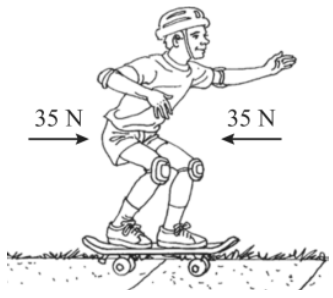
\includegraphics[width=6cm]{physics/figures/figure-unit-2-skater.png}
% \end{center}

\begin{center}
    \begin{tikzpicture}
        \draw (0,0) node {\reflectbox{\twemoji[height=2.5cm]{delivery truck}}};
        \draw[thick,<-,left=1.5cm] (0,0) -- (-4,0) node[above,pos=0.5] {400\,N};  
        \draw[thick,<-,right=1.5cm] (0,0) -- (+3,0) node[above,pos=0.5] {300\,N};  
    \end{tikzpicture}
\end{center}

\begin{randomizechoices}[norandomize]
    \correctchoice Moving and increasing their velocity, due to unbalanced forces.
    \choice Moving and decreasing their velocity, due to unbalanced forces.
    \choice Moving and increasing their velocity, up due to balanced forces.
    \choice Moving at a constant velocity, due to balanced forces.
\end{randomizechoices}


\question 
When a bug hits the windshield of a car traveling at \SI{40}{mph}, the force of the bug on the windshield is

\begin{randomizechoices}[norandomize]
    \choice Greater than the force of the windshield on the bug.
    \choice Less than the force of the windshield on the bug.
    \correctchoice The same as the force of the windshield on the bug.
\end{randomizechoices}

\question
A student measuring the velocity and time of a toy car wrote down the following data.

\begin{center}
    \begin{tabular}{|c|c|c|c|c|c|c|}
        \hline
        \textbf{Velocity} (m/s) & \SI{4}{m/s} &  \SI{4}{m/s} & \SI{2}{m/s} & \SI{2}{m/s} & \SI{2}{m/s} & \SI{2}{m/s} \\ \hline
        \textbf{Time} (s) & \SI{0}{s} & \SI{2}{s} & \SI{4}{s} & \SI{6}{s} & \SI{8}{s} & \SI{10}{s} \\
        \hline
    \end{tabular}
\end{center}

What happened during the time interval between 2--4 seconds?

\begin{randomizechoices}[norandomize]
    \choice An unbalanced force was applied to the car increasing the car’s velocity.
    \correctchoice An unbalanced force was applied to the car, decreasing the car’s velocity.
    \choice A balanced force was applied to the car increasing the car’s velocity.
    \choice A balanced force was applied to the car, decreasing the car’s velocity.   
\end{randomizechoices}


\question 
Which of the following graphs represents an object with no kinetic energy?

\begin{center}
    \begin{tikzpicture}
        \draw[->] (0,0) -- (0,2.5) node[above,rotate=90,pos=0.5] {Velocity (m/s)};
        \draw[->] (0,0) -- (2.5,0) node[below,pos=0.5] {Time (s)};
        \draw[ultra thick] (0,1.5) -- ++(2,0);
        \node at (1.25,2.8) {\textbf{Graph A}};
    \end{tikzpicture}
    \hspace{2em}
    \begin{tikzpicture}
        \draw[->] (0,0) -- (0,2.5) node[above,rotate=90,pos=0.5] {Velocity (m/s)};
        \draw[->] (0,0) -- (2.5,0) node[below,pos=0.5] {Time (s)};
        \draw[ultra thick] (0,0) -- (2,2);
        \node at (1.25,2.8) {\textbf{Graph B}};
    \end{tikzpicture}
    \hspace{2em}
    \begin{tikzpicture}
        \draw[->] (0,0) -- (0,2.5) node[above,rotate=90,pos=0.5] {Position (m)};
        \draw[->] (0,0) -- (2.5,0) node[below,pos=0.5] {Time (s)};
        \draw[ultra thick] (0,1.5) -- ++(2,0);
        \node at (1.25,2.8) {\textbf{Graph C}};
    \end{tikzpicture}
    \hspace{2em}
    \begin{tikzpicture}
        \draw[->] (0,0) -- (0,2.5) node[above,rotate=90,pos=0.5] {Position (m)};
        \draw[->] (0,0) -- (2.5,0) node[below,pos=0.5] {Time (s)};
        \draw[ultra thick] (0,2) -- (2,0);
        \node at (1.25,2.8) {\textbf{Graph D}};
    \end{tikzpicture}
\end{center}

\begin{randomizeoneparchoices}[norandomize]
    \choice Graph A
    \choice Graph B
    \correctchoice Graph C
    \choice Graph D
\end{randomizeoneparchoices}

\clearpage

\printkeytable


\end{questions}
\end{document}

